\chapter{Preparation for H(Inv) decays in the VBF channel with CMS parked data}
\label{CHAPTER:PreparationParkedDataAnalysis}

%%%%%%%%%%%%%%%%%%%%%%%%%%%%%%%%%%%%%%%%%%%%%%%%%%%%%%%%%%%%%%%%%%%%%%%%%%%%%%%%%%%%
%%% SECTION
%%%%%%%%%%%%%%%%%%%%%%%%%%%%%%%%%%%%%%%%%%%%%%%%%%%%%%%%%%%%%%%%%%%%%%%%%%%%%%%%%%%%
\section{L1T Parked Trigger Development}
\label{SECTION:ParkedDataAnalysis_ParkedTriggerDevelopment}

%Status: DONE

The first step of any analysis is defining or selecting a trigger to collect data. This trigger should have a high signal efficiency while recording an acceptable rate.

At the beginning of 2012 the possibility of recording data without promptly reconstructing it was introduced. This additional data is now known as \textit{parked data}. The \gls{CMS} \gls{VBF} Higgs to invisible analysis saw this as an opportunity to develop a secondary set of triggers with lower thresholds to allow more signal to be collected when compared with the developed prompt trigger. As this effort developed it became clear that an inclusive trigger that would record \gls{VBF} events regardless of final state could be implemented.

%%%%%%%%%%%%%%%%%%%%%%%%%%%%%%%%%%%%%%%%%%%%%%%%%%%%%%%%%%%%%%%%%%%%%%%%%%%%%%%%%%%%
%%% SUBSECTION
%%%%%%%%%%%%%%%%%%%%%%%%%%%%%%%%%%%%%%%%%%%%%%%%%%%%%%%%%%%%%%%%%%%%%%%%%%%%%%%%%%%%
\subsection{VBF Higgs to Invisible Higgs Trigger}
\label{SUBSECTION:ParkedDataAnalysis_ParkedTriggerDevelopment_VBFHiggsInvisibleTrigger}

%Status: DONE

This study was based on data recorded during the high \gls{PU} special run that happened in late 2011 and was aimed at making a proposal for a viable \gls{L1T} trigger algorithm to be used during the 2012 proton run. 

The investigated algorithms select the typical topology of our signal. They look for events with \gls{MET} and and two jets located in opposite sides of the detector by requiring $\eta_{jet1}\times\eta_{jet2}<0$, large pseudo-rapidity separation of at least $\Delta\eta_{jj}>3$. The possibility of using $\Delta\phi_{jj}$ was also studied but was disfavoured since it could lead to lower signal efficiency in some \gls{BSM} models.

The conditions expected for early 2012 were of instantaneous luminosity of $5 \times 10^{33}\,\centi\meter^{-2}\second^{-1}$ and an average \gls{PU} of 28 interactions (scenario A). For late 2012 conditions were expected to increase to instantaneous luminosity of $7 \times 10^{33}\,\centi\meter^{-2}\second^{-1}$ and an average \gls{PU} of 32 interactions (scenario B).

Algorithm parameters we optimized for both this scenarios of \gls{LHC} running and considering several benchmark \gls{L1T} rates. The proposed target rate for the algorithm was assumed to be $2\,\kilo\Hz$, the additional working points were calculated with the intention to adjust the selection cuts according to higher or lower bandwidth available on the menu. The two key variables are $\pt^{\text{jets}}$ and the \gls{MET}. Each of these variables was set in turn to the lowest reasonable value while the other was scanned until the necessary rate value was achieved.  Results for scenario A can be found in table \ref{TABLE:ParkedDataAnalysis_L1TParkedTriggerDevelopment_Rate5E33} and for scenario B in table \ref{TABLE:ParkedDataAnalysis_L1TParkedTriggerDevelopment_Rate7E33}.

\begin{table}[!htb]
\begin{minipage}{.5\linewidth}
  \centering
  \begin{tabular}{|c||c|c|c|c|}
  \hline
  \multicolumn{5}{|c|}{MET [GeV] ($\pt^{\text{jets}} > 20\,\GeV$)} \\
  \hline\hline
  $\Delta\phi$ & no cut & 2.5 & 2.1 & 1.8 \\
  \hline
   $10\,\kHz$  &     32 &  32 &  32 &  32 \\
    $5\,\kHz$  &     35 &  35 &  35 &  35 \\
  \hline\hline
    $2\,\kHz$  &     41 &  41 &  41 &  41 \\
  \hline\hline
    $1\,\kHz$  &     47 &  47 &  47 &  46 \\
  $0.5\,\kHz$  &     54 &  54 &  54 &  53 \\
  \hline
  \end{tabular}
\end{minipage}%
\begin{minipage}{.5\linewidth}
  \centering
  \begin{tabular}{|c||c|c|c|c|}
  \hline
  \multicolumn{5}{|c|}{$\pt^{\text{jets}}$ [GeV] ($\text{MET}>30\,\GeV$)} \\
  \hline
  $\Delta\phi$ & no cut & 2.5 & 2.1 & 1.8 \\
  \hline\hline
   $10\,\kHz$  &     28 &  28 &  24 &  24 \\
    $5\,\kHz$  &     32 &  32 &  32 &  32 \\
  \hline\hline
    $2\,\kHz$  &     52 &  48 &  44 &  44 \\
  \hline\hline
    $1\,\kHz$  &     68 &  68 &  64 &  64 \\
  $0.5\,\kHz$  &     92 &  92 &  88 &  88 \\
  \hline
  \end{tabular}
\end{minipage} 
\caption{Tables showing the \gls{L1T} rate for different selection criteria for $5 \times 10^{33}\,\centi\meter^{-2}\second^{-1}$ and an average \gls{PU} of 28 interactions (scenario A). In selected events the leading two jets is in opposite sides of the detector. On the left table the \gls{MET} cut is calculated while requiring the two leading jets to have $\pt^{\text{jets}} > 20\,\GeV$. Similarly, on the right table $\pt^{\text{jets}}$ cut is calculated while requiring $\text{MET}>30\,\GeV$.}
\label{TABLE:ParkedDataAnalysis_L1TParkedTriggerDevelopment_Rate5E33}
\end{table}

\begin{table}[!htb]
\begin{minipage}{.5\linewidth}
  \centering
  \begin{tabular}{|c||c|c|c|c|}
  \hline
  \multicolumn{5}{|c|}{MET [GeV] ($\pt^{\text{jets}}>20\,\GeV$)} \\
  \hline\hline
  $\Delta\phi$ & no cut & 2.5 & 2.1 & 1.8 \\
  \hline
   $10\,\kHz$  &     36 &  36 &  36 &  36 \\
    $5\,\kHz$  &     40 &  40 &  40 &  40 \\
  \hline\hline
    $2\,\kHz$  &     47 &  47 &  47 &  46 \\
  \hline\hline
    $1\,\kHz$  &     54 &  54 &  54 &  54 \\
  $0.5\,\kHz$  &     67 &  66 &  66 &  64 \\
  \hline
  \end{tabular}
\end{minipage}%
  \begin{minipage}{.5\linewidth}
    \centering
  \begin{tabular}{|c||c|c|c|c|}
  \hline
  \multicolumn{5}{|c|}{$\pt^{\text{jets}}$ [GeV] ($\text{MET}>30\,\GeV$)} \\
  \hline
  $\Delta\phi$ & no cut & 2.5 & 2.1 & 1.8 \\
  \hline\hline
   $10\,\kHz$  &     32 &  32 &  32 &  32 \\
    $5\,\kHz$  &     40 &  40 &  40 &  40 \\
  \hline\hline
    $2\,\kHz$  &     64 &  60 &  60 &  56 \\
  \hline\hline
    $1\,\kHz$  &     76 &  76 &  76 &  76 \\
  $0.5\,\kHz$  &    100 & 100 &  96 &  92 \\
  \hline
  \end{tabular}
\end{minipage} 
\caption{Tables showing the \gls{L1T} rate for different selection criteria for $7 \times 10^{33}\,\centi\meter^{-2}\second^{-1}$ and an average \gls{PU} of 32 interactions (scenario B). In selected events the leading two jets is in opposite sides of the detector. On the left table the \gls{MET} cut is calculated while requiring the two leading jets to have $\pt^{\text{jets}} > 20\,\GeV$. Similarly, on the right table $\pt^{\text{jets}}$ cut is calculated while requiring $\text{MET}>30\,\GeV$.}
\label{TABLE:ParkedDataAnalysis_L1TParkedTriggerDevelopment_Rate7E33}
\end{table}

These results were used to define working points for this trigger, which were proposed to the \glsreset{TSG}
to be included on \gls{L1T} Menus. Proposed trigger options were:
\begin{itemize}
\item Algorithm A: Lead dijet (opp. sides + $\pt^{\text{jets}}>20\,\GeV$ + $\Delta\eta_{jj}>3$) + $\text{MET}>40\,\GeV$
\item Algorithm B: Lead dijet (opp. sides + $\pt^{\text{jets}}>50\,\GeV$ + $\Delta\eta_{jj}>3$) + $\text{MET}>30\,\GeV$
\end{itemize}

It can be observed that with the at the time predicted increase of luminosity the necessary rate for such proposed algorithms could escalate to $\approx 5\,\kilo\Hz$. For the rate to be maintained at $2\,\kilo\Hz$ the value of the MET cut in algorithm A would have to be raised to $47\,\GeV$ and the value of $\pt^{\text{jets}}$ cut in algorithm B would have to increase to $64\,\GeV$.

%%%%%%%%%%%%%%%%%%%%%%%%%%%%%%%%%%%%%%%%%%%%%%%%%%%%%%%%%%%%%%%%%%%%%%%%%%%%%%%%%%%%
%%% SUBSECTION
%%%%%%%%%%%%%%%%%%%%%%%%%%%%%%%%%%%%%%%%%%%%%%%%%%%%%%%%%%%%%%%%%%%%%%%%%%%%%%%%%%%%
\subsection{VBF Higgs Inclusive Trigger}
\label{SUBSECTION:ParkedDataAnalysis_ParkedTriggerDevelopment_InclusiveHiggsTrigger}

It would be desirable to have a dedicated \gls{VBF} Higgs inclusive \gls{L1T} trigger that would be decay independent. Such an algorithm would allow analysts to have a single trigger for all \gls{VBF} produced Higgs decay signatures, which would implies less systematics in their comparison. Additionally, if an algorithm is used by more analysis it will become better understood.

When selecting events based only on the presence of a dijet with \gls{VBF} characteristics we can remove the dependency on the Higgs decay. This approach would be suitable since it ignores the Higgs decays themselves. Since we are not making any assumptions of the Higgs model, we could study all possible decays even those predicted by new models with a single trigger. Thus, it would be a model-independent trigger.

This trigger can also be used for a WW scattering analysis, which in the case of the absence of the now discovered Higgs boson would allow to eventually exclude the standard model.


%%TODO: Below

For such a trigger to work it would have to be based only on the forward dijet which is the defining caracteristic
of the VBF signature.
It was decided to study two variables of the dijet system: invariant mass and transverse invariant mass (MT); and an event 
variable, scalar sum of the hadronic energy (HT). For this study we always require a dijet with $\Delta\eta>3$ and we 
look at the effects of an additional cut on $\Delta\phi$, the points tested were no cut, $<2.5$, $<2.1$ and $<1.8$.

\subsubsection{Dijet invariant mass}

This variable takes advantage from the very high invariant mass of the dijet system but it is not yet implemented
on the L1 hardware but according to trigger experts it is in principle possible to implement with the current hardware.

Unfortunately, using this variable alone to is not enough. To get acceptable rates we would need to cut too high on
jet $p_\bot$ or $M_{Inv}$ losing almost all signal efficiency.

\subsubsection{Dijet transverse invariant mass}

This variable is better at suppressing QCD events, it is less pileup-dependent and has lower error associated with it
(only x-y dependence). It is also not yet implemented on the L1 Hardware but according to trigger experts it is in principle 
possible to implement with the current hardware.

This variable showed to be promising. A possible working point for a Level 1 rate
of 5kHz could be $MT>50$ $GeV$ no $\Delta\phi$ cut and dijet $p_\bot \sim 45$ $GeV$ which should give a signal
efficiency of $\lesssim70\%$ (see R. Lane 3 Months PhD Report).

\subsubsection{Event scaler sum of the transverse energy}

Theoretically, this is the best variable to separate signal from background and has the advantage of being already
implemented on L1 hardware.

This was shown to be the most promising variable. A possible working point for a Level 1 rate of 5kHz could be $HT>100$ 
$GeV$ no $\Delta\phi$ cut and dijet $p_\bot \sim 40$ $GeV$ which should give a signal efficiency of $\lesssim98\%$
(see Figures \ref{figure_PU28_5e33_RateFBDijetDEtaDPhi00HT100} and \ref{figure_sig_eff_l1_ht}).

\begin{figure}[ht]
\centering
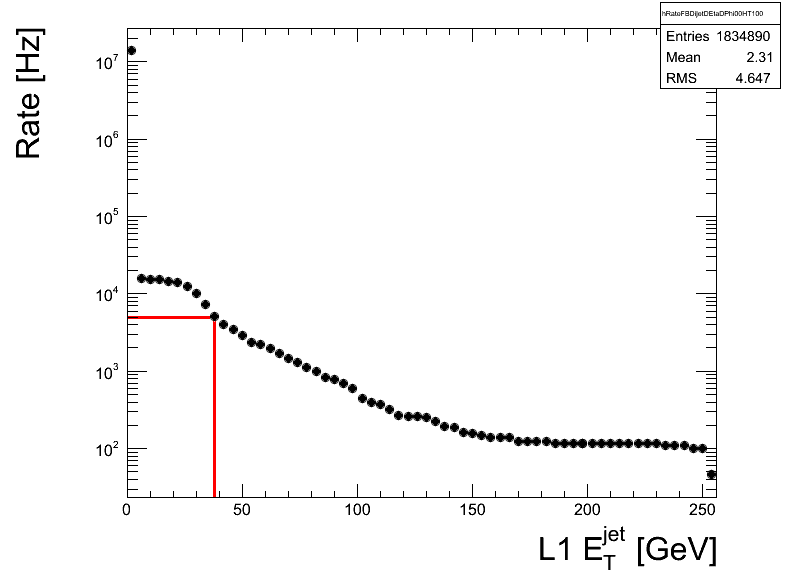
\includegraphics[width=0.60\textwidth]{Chapter07/ParkedDataTriggerDevelopment/Images/PU28_5e33_RateFBDijetDEtaDPhi00HT100.png}
\caption{Level 1 rate as a function of dijet $p_\bot$ while selecting events with $HT>100$ $GeV$. Results based on
data from the high pileup special run taken late 2011.}
\label{figure_PU28_5e33_RateFBDijetDEtaDPhi00HT100}
\end{figure}

\subsection{Final proposal}

%%%%%%%%%%%%%%%%%%%%%%%%%%%%%%%%%%%%%%%%%%%%%%%%%%%%%%%%%%%%%%%%%%%%%%%%%%%%%%%%%%%%
%%% SECTION
%%%%%%%%%%%%%%%%%%%%%%%%%%%%%%%%%%%%%%%%%%%%%%%%%%%%%%%%%%%%%%%%%%%%%%%%%%%%%%%%%%%%
\section{QCD VBF+MET Monte Carlo simulation}

\begin{table}
\centering
\begin{tabular}{|c|r|c|r|c|c|}
  \hline
  Sample          &       Ev. Gen. & Filter Eff. &  Events &  XS $[pb]$ & Eq. Lumi. $[fb^{-1}]$ \\
  \hline \hline
  QCD-Pt-80to120  & 39376000000 &    0.000049 & 1614416 &  1033680 &  38.09 \\
  QCD-Pt-120to170 &  7000000000 &    0.000283 & 2051000 & 156293.3 &  44.79 \\
  QCD-Pt-170to300 &  1375000000 &    0.000987 & 1391500 & 34138.15 &  40.28 \\
  QCD-Pt-300to470 &    80000000 &    0.002659 &  207840 & 1759.549 &  45.47 \\
  QCD-Pt-470to600 &    25000000 &    0.004127 &  104675 & 113.8791 & 219.53 \\
  \hline
\end{tabular}
\end{table}

\begin{figure}[h!]
\centering
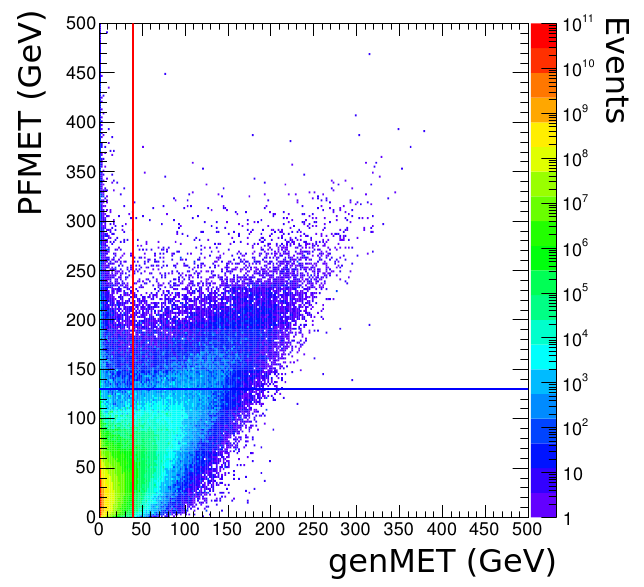
\includegraphics[width=0.55\textwidth]{Chapter05/ParkedDataPreparation/Images/Joao_140209_p11.png}
\caption{Reconstructed PFMET as a function of generator-level MET
      in the inclusive QCD samples $80 < \hat{p_T} < 600$ GeV before
      any selection.}
\label{fig:qcdRecovsGenMET}
\end{figure}

\section{Dijet-MET system topological variables}


\section{Track distribution variables}


% %%%%%%%%%%%%%%%%%%%%%%%%%%%%%%%%%%%%%%%%%%%%%%%%%%%%%%%%%%
% Jet topology variables
% %%%%%%%%%%%%%%%%%%%%%%%%%%%%%%%%%%%%%%%%%%%%%%%%%%%%%%%%%%
% 18 Months report was on the Sep 9 2013
% 
% /home/hep/jca10/work/vbfinv/ws04/CMSSW_5_3_11/src/UserCode/ICHiggsTauTau/Analysis/HiggsNuNu/PLOTS_mjj1200_dijetFrac/nunu/MET130/n_vtx_2012_DijetFraction_log.pdf
% Looks like plots are from Jun 25 2013
% 
% FOUND FILE: This is the file used in the plots for the 18 months report
% /home/hep/jca10/work/vbfinv/ws04/CMSSW_5_3_11/src/UserCode/ICHiggsTauTau/Analysis/HiggsNuNu/output_mjj1100_dijetFrac/nunu/MET130/MC_VBF_HToZZTo4Nu_M-120.root
% 
% /vols/cms02/jca10/work/ws01/CMSSW_5_3_11/src/UserCode/ICHiggsTauTau/Analysis/HiggsNuNu/plots/DPhiSIGNAL_CJVpass/dijetMet/dijetFrac_htMET.png
% Looks like plots are from Feb 20 2014


% %%%%%%%%%%%%%%%%%%%%%%%%%%%%%%%%%%%%%%%%%%%%%%%%%%%%%%%%%%
% Track variables
% %%%%%%%%%%%%%%%%%%%%%%%%%%%%%%%%%%%%%%%%%%%%%%%%%%%%%%%%%%
% 20140603_ICVBFHiggs_JPela.pdf
% /afs/cern.ch/user/p/pela/work/cms/vbfinv/ws03/CMSSW_5_3_11/src/VBFHiggsToInvisible/VariableAnalyser/python/PowhegSignal_cfi.py
% 
% %%%%%%%%%%%%%%%%%%%%%%%%%%%%%%%%%%%%%%%%%%%%%%%%%%%%%%%%%%
% QCD VFB + MET samples
% %%%%%%%%%%%%%%%%%%%%%%%%%%%%%%%%%%%%%%%%%%%%%%%%%%%%%%%%%%
% 20140204_ICVBFHiggs_JPela_VBFQCD.pdf (plot on the AN)
% 20140506_ICVBFHiggs_JPela.pdf (selection test)
% 
% Something odd here
% /home/hep/jca10/work/vbfinv/ws08/CMSSW_5_3_11/src/UserCode/ICHiggsTauTau/Analysis/HiggsNuNu

%%%%%%%%%%%%%%%%%%%%%%%%%%%%%%%%%%%%%%%%%%%%%%%%%%%%%%%%%%%%%%%%%%%%%%%%%%%%%%%%%%%
%%%%%%%%%%%%%%%%%%%%%%%%%%%%%%%%%%%%%%%%%%%%%%%%%%%%%%%%%%%%%%%%%%%%%%%%%%%%%%%%%%%
%%%%%%%%%%%%%%%%%%%%%%%%%%%%%%%%%%%%%%%%%%%%%%%%%%%%%%%%%%%%%%%%%%%%%%%%%%%%%%%%%%%

